
% If the calculus has an acronym, define it.
% (e.g. \newcommand{\LK}{\ensuremath{\mathbf{LK}}\xspace})

\calculusName{System GK}   % The name of the calculus
\calculusAcronym{\GK}    % The acronym if defined above, or empty otherwise. 
\calculusLogic{Modal}  % Specify the logic (e.g. classical, intuitionistic, ...) for which this calculus is intended.
\calculusType{Sequent Calculus}   % Specify the calculus type (e.g. Frege-Hilbert style, tableau, sequent calculus, hypersequent calculus, natural deduction, ...)
\calculusYear{1998}   % The year when the calculus was invented.
\calculusAuthor{Hiroakira Ono} % The name(s) of the author(s) of the calculus.

\entryTitle{Sequent Calculus for Basic Modal Logics} % Title of the entry (usually coincides with the name of the calculus).
\entryAuthor{Harley Eades III \and Valeria de Paiva} % Your name(s). Separate multiple names with "\and".

% If you wish, use tags to give any other information 
% that might be helpful for classifying and grouping this entry:
% e.g. \tag{Two-Sided Sequents}
% e.g. \tag{Multiset Cedents}
% e.g. \tag{List Cedents}
% You are free to invent your own tags. 
% The Encyclopedia's coordinator will take care of 
% merging semantically similar tags in the future.
\tag{Two-Sided Sequents}

\maketitle

% If your files are called "MyProofSystem.tex" and "MyProofSystem.bib", 
% then you should write "\begin{entry}{MyProofSystem}" in the line below
\begin{entry}{GK}  

% Define here any newcommands you may need:
% e.g. \newcommand{\necessarily}{\Box}
% e.g. \newcommand{\possibly}{\Diamond}

\begin{calculus}
  \[
  \begin{array}{lll}
    \text{Version 0:}\\
    & \begin{array}{ccc}
        \infer[\Box]{\Box \Gamma \vdash \Box A}{\Gamma \vdash A}    
      \end{array}
    \\\\
    \text{Version 1:}\\
    & \begin{array}{ccc}
        \infer[\Box_l]{\Box A,\Gamma \vdash \Delta}{A,\Gamma \vdash \Delta}
        & \quad &
        \infer[\Box_r]{\Box \Gamma \vdash \Box A}{\Box \Gamma \vdash A}
      \end{array}
    \\\\
    \text{Version 2:}\\
    & \begin{array}{ccc}
        \infer[\Box_l]{\Box A,\Gamma \vdash \Delta}{A,\Gamma \vdash \Delta}
        & \quad &
        \infer[\Box_r]{\Box \Gamma \vdash \Box A,\Box \Delta}{\Box \Gamma \vdash A,\Box \Delta}
      \end{array}
  \end{array}
  \]
\end{calculus}

% The following sections ("clarifications", "history", 
% "technicalities") are optional. If you use them, 
% be very concise and objective. Nevertheless, do write full sentences. 
% Try to have at most one paragraph per section, because line breaks 
% do not look nice in a short entry.

\begin{clarifications}
There are three equivalent versions of system GK \cite{Ono:1998} which
are extensions of LK \iref{GentzenLK}.  That is, version 0 consists of
the rules of LK in addition to the rule given above, and similarly for
the remaining two systems.  Version 2 can derive the rules of version
1, and version 1 can derive the rules in version 0.  Lastly, $\Gamma$
and $\Delta$ are multisets of formulas where $\Box \Gamma$
(resp. $\Box \Delta$) is equivalent to applying $\Box$ to each formula
in $\Gamma$ (resp. $\Delta$).
\end{clarifications}

\begin{history}
%% ToDo: write here short historical remarks about this proof system,
%% especially if they relate to other proof systems. 
%% Use "\iref{OtherProofSystem}" to refer to another proof system 
%% in the Encyclopedia (where "OtherProofSystem" is its ID). 
%% Use "\irefmissing{SuggestedIDForOtherProofSystem}" to refer to 
%% another proof system that is not yet available in the encyclopedia.
The original sequent calculus version for the Lewis systems S4, S5
appear in Ohnishi and Matsumoto 52, 57, who credit Curry for the S4
only version \cite{Ohnishi:1957,Ohnishi:1959}. Since at least the late
50s it was clear that systems of modal logic should be considered
together, a tradition that has given us the modal cube below. The
realization that the basic system should be the system K, named for
Kripke, only became clear later on. A clear discussion of system K can
be found in Ono \cite{Ono:1998}.

\begin{figure}
  \begin{center}
    \scalebox{0.8}{
    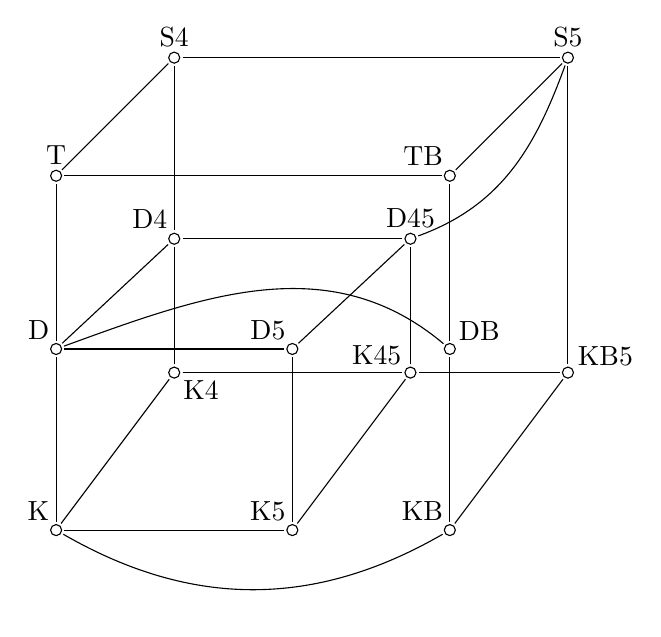
\begin{tikzpicture}[every node/.style={inner sep=0,outer sep=1}]
  %% Right node in upper rect.
  \node[circle,draw,minimum size=4pt,label=T] (P1) at (-1.5,0) {};
  \node[circle,draw,minimum size=4pt,label=S4] (P2) at (0,1.5) {};
  %% Left nodes in upper rect.
  \node[circle,draw,minimum size=4pt,label=120:TB] (P3) at (3.5,0) {};
  \node[circle,draw,minimum size=4pt,label=S5] (P4) at (5,1.5) {};
  %% 
  \node[circle,draw,minimum size=4pt,label=120:K] (P5) at (-1.5,-4.5) {};
  \node[circle,draw,minimum size=4pt,label=-40:K4] (P6) at (0,-2.5) {};
  %% 
  \node[circle,draw,minimum size=4pt,label=120:KB] (P7) at (3.5,-4.5) {};
  \node[circle,draw,minimum size=4pt,label=30:KB5] (P8) at (5,-2.5) {};
  %% 
  \node[circle,draw,minimum size=4pt,label=120:D] (P9) at (-1.5,-2.2) {};
  \node[circle,draw,minimum size=4pt,label=120:D4] (P10) at (0,-0.8) {};


  \node[circle,draw,minimum size=4pt,label=120:K5] (P11) at (1.5,-4.5) {};
  \node[circle,draw,minimum size=4pt,label=120:D5] (P12) at (1.5,-2.2) {};

  \node[circle,draw,minimum size=4pt,label=140:K45] (P13) at (3,-2.5) {};
  \node[circle,draw,minimum size=4pt,label=D45] (P14) at (3,-0.8) {};

  \node[circle,draw,minimum size=4pt,label=40:DB] (P15) at (3.5,-2.2) {};
  
  \draw (P1) -- (P2);
  \draw (P2) -- (P4);
  \draw (P1) -- (P3);
  \draw (P3) -- (P4);

  \draw (P6) -- (P13) -- (P8);
  \draw (P5) -- (P6);
  \draw (P5) -- (P11);
  \draw (P5) to [out=-30,in=-150] (P7);
  \draw (P7) -- (P8);

  \draw (P5) -- (P9)  -- (P1);  
  \draw (P6) -- (P10) -- (P2);
  \draw (P4) -- (P8);
  \draw (P3) -- (P15) -- (P7);

  \draw (P9) -- (P10);
  \draw (P9) -- (P12);
  \draw (P11) -- (P12);
  \draw (P11) -- (P13);
  \draw (P13) -- (P14);
  \draw (P10) -- (P14);
  \draw (P12) -- (P14);
  \draw (P14) to [out=20,in=-110] (P4);

  \draw (P9) to [out=20,in=140] (P15);
\end{tikzpicture}}
\end{center}
  \caption{Modal Cube}
  \label{fig:modal-cube}
\end{figure}

\end{history}

% General Instructions:
% =====================

% The preferred length of an entry is 1 page. 
% Do the best you can to fit your proof system in one page.
%
% If you are finding it hard to fit what you want in one page, remember:
%
%   * Your entry needs to be neither self-contained nor fully understandable
%     (the interested reader may consult the cited full paper for details)
%
%   * If you are describing several proof systems in one entry, 
%     consider splitting your entry.
%
%   * You may reduce the size of your entry by ommitting inference rules
%     that are already described in other entries.
%
%   * Cite parsimoniously (see detailed citation instructions below).
%
% 
% If you do not manage to fit everything in one page, 
% it is acceptable for an entry to have 2 pages.
%
% For aesthetical reasons, it is preferable for an entry to have
% 1 full page or 2 full pages, in order to avoid unused blank space.



% Citation Instructions:
% ======================

% Please cite the original paper where the proof system was defined.
% To do so, you may use the \cite command within 
% one of the optional environments above,
% or use the \nocite command otherwise.

% You may also cite a modern paper or book where the 
% proof system is explained in greater depth or clarity.
% Cite parsimoniously.

% Do not cite related work. Instead, use the "\iref" or "\irefmissing" 
% commands to make an internal reference to another entry, 
% as explained within the "history" environment above.

% You do not need to create the "References" section yourself. 
% This is done automatically.




% Leave an empty line above "\end{entry}".

\end{entry}
